\documentclass{beamer}
%~ \usetheme{Hannover}  %% Themenwahl
%~ \usetheme{Bergen}  %% Themenwahl
\usetheme{Berkeley}  %% Themenwahl
\usecolortheme{dove}

\usepackage[utf8]{inputenc}
\usepackage[T1]{fontenc}

\usepackage[english]{babel}

\usepackage{graphicx}
\usepackage{upgreek}
\usepackage{float}
\usepackage{units}
\usepackage{url}

\usepackage{amsmath}
\usepackage{amssymb}
\usepackage{amsfonts}

\usepackage{longtable}

\usepackage{ae}
\usepackage{booktabs}

\usepackage{tikz}
\usetikzlibrary{patterns}

%\abs{Ausdruck} %Betragsstriche, die skalieren - abgekürzt
\newcommand{\abs}[1]{\ensuremath{\left\vert#1\right\vert}}
% und das gleiche füur große Klammern
\newcommand{\brac}[1]{\ensuremath{\left(#1\right)}}
% Erwartungswert skalierend
\newcommand{\avg}[1]{\left< #1 \right>}
% ein nicht kursives d für Ableitungen/Integrale, mit etwas Platz davor, um sich etwas abzusetzten
\newcommand{\de}{\ensuremath{\,\mathrm{d}}}
% Für Einheiten: schreibt sie nicht kursiv und lässt etwas Platz zur Zahl vorher
\newcommand{\eh}[1]{\ensuremath{\,\mathrm{#1}}}
% einfaches Gradzeichen
\newcommand{\gr}{\ensuremath{^{\circ}}}
% Fehlerfortpfanzung
% dy/dz * delta z
\newcommand{\fehler}[2]%
{\ensuremath{\abs{\frac{\partial #1}{\partial #2}}\cdot \Delta #2}}

\title{Ising-Ferromagnet auf Ad-Hoc Netzwerken}
\author{Hendrik Schawe}
\date{\today}

\begin{document}

\maketitle
\frame{\tableofcontents[pausesections]}

\section{Model}
    \subsection{Ising Ferromagnet}
        \begin{frame}{Ising Ferromagnet}
            \begin{itemize}[<+->]
                \item \(N\) sites
                \item \(\avg{i,j}\) denotes "nearest neighbor" relationship
                \item every site has a spin \(s \in \{-1,+1\}\){}
                \item two spins \(i,j\) are coupled by \(J_{ij}\)
                \item{
                    \begin{equation}
                        H = - \sum_{\avg{i,j}}J_{ij}s_{i}s_{j}.
                    \end{equation}
                    (Ref.\ \cite{Ising1925})
                }
            \end{itemize}
        \end{frame}

        \begin{frame}{Disordered Ising Ferromagnet}
            \begin{columns}[t]
                \begin{column}{5cm}
                    \begin{itemize}
                        \item<1-> start with square lattice
                        \item<2-> displace every node randomly according to\\
                            \(f(x)=\frac{1}{\sqrt{2\pi}\sigma}\mathrm{e}^{-\frac{x^2}{2\sigma^2}}.\){}
                        \item<3-> assign new nearest neighbors
                        \item<4-> depending on their distance \(d_{ij}\) assign new \(J_{ij} = e^{\alpha(1-d_{ij})}\)
                        \item<4-> here \(\alpha = 0.5\)
                    \end{itemize}
                \end{column}
                \begin{column}{6cm}
                    \visible<2->{
                        \vspace{-1cm}
                        \begin{figure}[htbp]
                            \centering
                            \begin{tikzpicture}[scale=1.5, declare function={
        normal(\x,\m,\y) = 1/2/exp((\x-\m)*(\x-\m)/2/(\s^2))-\y;
      }]
    \def\s{0.5}

    \draw[dotted] (-2,0) -- (4,0);
    \draw[dotted] (0,-2) -- (0,2);
    \draw[dotted] (2,-2) -- (2,2);

    % Draw and label normal distribution function
    \def\dxa{0.4}
    \def\dya{-0.8}

    \draw (0+\dxa,0+\dya) -- node [right] {$\Delta x$} (0+\dxa, {normal(\dxa,0,0)});
    \draw (0+\dxa,0+\dya) -- node [below] {$\Delta y$} ({-normal(\dya,0,0)}, 0+\dya);
    \draw[->] (0,0) -- (0+\dxa*0.9,0+\dya*0.9);

    \draw[color=black,domain=-1.5:1.5] plot [smooth] (\x,{normal(\x,0,0)}) node[right] {};
    \fill (0, 0) circle(0.08);
    \draw[color=black] (0+\dxa, 0+\dya) circle(0.08);
    \draw[color=black,domain=-1.5:1.5,rotate=90] plot [smooth] (\x,{normal(\x,0,0)}) node[right] {};


    \def\dxb{0.5}
    \def\dyb{0.2}

    \draw[color=red] (2+\dxb,0+\dyb) -- node [right] {$\Delta x_{2}$} (2+\dxb, {normal(\dxb,0,0)});
    \draw[color=red] (2+\dxb,0+\dyb) -- node [below] {$\Delta y_{2}$} ({2-normal(\dyb,0,0)}, 0+\dyb);
    \draw[color=red,->] (2,0) -- (2+\dxb*0.9,0+\dyb*0.9);

    \draw[color=red,domain=0.5:3.5] plot [smooth] (\x,{normal(\x,2,0)}) node[right] {};
    \fill[color=red] (2, 0) circle(0.08);
    \draw[color=red] (2+\dxb, 0+\dyb) circle(0.08);
    \draw[color=red,domain=-1.5:1.5,rotate=90] plot [smooth] (\x,{normal(\x,0,2)}) node[right] {};
\end{tikzpicture}

                            \caption
                            {
                                Displacement of the nodes.
                            }
                        \end{figure}
                    }
                \end{column}
            \end{columns}
        \end{frame}

    \subsection{Proximity Graphs}
        \begin{frame}{Proximity Graphs}
            \begin{itemize}[<+->]
                \item{ 3 graph types used
                    \begin{itemize}
                        \item Delaunay Triangulation (DT) \cite{Katajainen}
                        \item Gabriel Graph (GG) \cite{Gabriel1969}
                        \item Relative Neighborhood Graph (RNG) \cite{Toussaint1980}
                    \end{itemize}
                }
                \item{
                    \begin{equation}
                        DT \supseteq GG \supseteq RNG
                    \end{equation}
                }
            \end{itemize}
        \end{frame}

        \begin{frame}{Delaunay Triangulation}
            \begin{figure}[htbp]
                \centering
                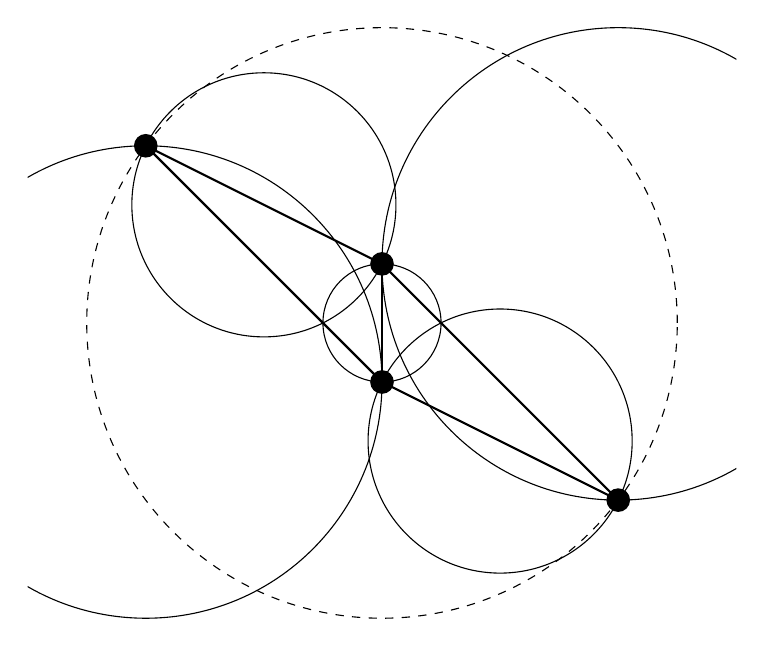
\begin{tikzpicture}[scale=3]
    \clip (-0.5,0) rectangle (2.5,2.5);

    \fill (0, 2  ) circle(0.05);
    \fill (1, 1.5) circle(0.05);
    \fill (1, 1  ) circle(0.05);
    \fill (2, 0.5) circle(0.05);

    \draw[dashed] (1, 1.25)   circle(1.25);
    \draw (2, 1.5)      circle(1);
    \draw (1, 1.25)     circle(0.25);
    \draw (0.5, 1.75)   circle(0.5590);
    \draw (1.5, 0.75)   circle(0.5590);
    \draw (0, 1)        circle(1);

    \draw[thick] (0, 2  ) -- (1, 1.5);
    \draw[thick] (0, 2  ) -- (1, 1  );
    \draw[thick] (1, 1  ) -- (1, 1.5);
    \draw[thick] (1, 1  ) -- (2, 0.5);
    \draw[thick] (1, 1.5) -- (2, 0.5);
\end{tikzpicture}

                \caption
                {
                    Example of a DT.
                }
            \end{figure}
        \end{frame}

        \begin{frame}{Gabriel Graph}
            \begin{columns}[b]
                \begin{column}{5cm}
                    \begin{figure}[htbp]
                        \centering
                        \documentclass{standalone}

\usepackage{tikz}
\usetikzlibrary{arrows}

\begin{document}
    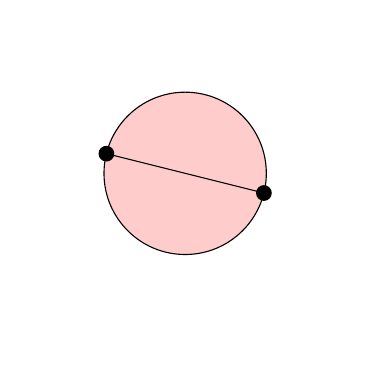
\begin{tikzpicture}
        \clip (-2,2.1) rectangle (2,-2);

        \fill[fill=red!20] (0, 0.25) circle(1.0307764064);
        \draw (0, 0.25) circle(1.0307764064);
        %~ \pattern[pattern color=black!60, pattern=north west lines];


        \fill (-1, 0.5) circle(0.1);
        \fill (1, 0) circle(0.1);
        \draw (1, 0) -- (-1, 0.5);
    \end{tikzpicture}
\end{document}

                        \caption
                        {
                            Lune of a GG.
                        }
                    \end{figure}
                \end{column}
                \begin{column}{5cm}
                    \begin{figure}[htbp]
                        \centering
                        \includegraphics[width=1\textwidth]{images/GG/L12S03.pdf}
                        \caption
                        {
                            GG Example
                        }
                    \end{figure}
                \end{column}
            \end{columns}
        \end{frame}

        \begin{frame}{Relative Neighborhood Graph}
            \begin{columns}[b]
                \begin{column}{5cm}
                    \begin{figure}[htbp]
                        \centering
                        \documentclass{standalone}

\usepackage{tikz}
\usetikzlibrary{arrows}

\begin{document}
    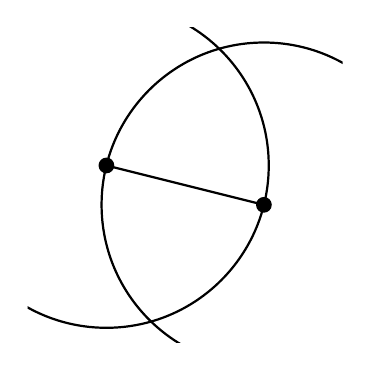
\begin{tikzpicture}
        \clip (-2,2.25) rectangle (2,-1.75);

        \begin{scope}
            \clip (-1, 0.5) circle(2.06155281281);
            \draw (1, 0) circle(2.06155281281);
        \end{scope}

        \draw[thick] (-1, 0.5) circle(2.06155281281);
        \fill (-1, 0.5) circle(0.1);
        \draw[thick] (1, 0) circle(2.06155281281);
        \fill (1, 0) circle(0.1);
        \draw[thick] (1, 0) -- (-1, 0.5);
    \end{tikzpicture}
\end{document}

                        \caption
                        {
                            Lune of a RNG.
                        }
                    \end{figure}
                \end{column}
                \begin{column}{5cm}
                    \begin{figure}[htbp]
                        \centering
                        \includegraphics[width=1\textwidth]{images/RNG/L12S03.pdf}
                        \caption
                        {
                            RNG Example
                        }
                    \end{figure}
                \end{column}
            \end{columns}
        \end{frame}

        \begin{frame}{Graph Generation}
            \begin{columns}[t]
                \begin{column}{5cm}
                    \begin{itemize}
                        \item<1-> Fastest: generate DT in \(O(n \log(n))\) and test every edge
                        \item<2-> But DT generation is not trivial
                        \item<3-> Simplest: test every possible edge in \(O(n^{3})\)
                        \item<4-> But: really slow
                        \item<5-> Idea: test only nodes near the lune for every pair in best case \(O(n^{2})\)
                    \end{itemize}
                \end{column}
                \begin{column}{5cm}
                    \begin{overprint}
                        \onslide<6>{
                            \only<6>{
                                \begin{figure}[htbp]
                                    \centering
                                    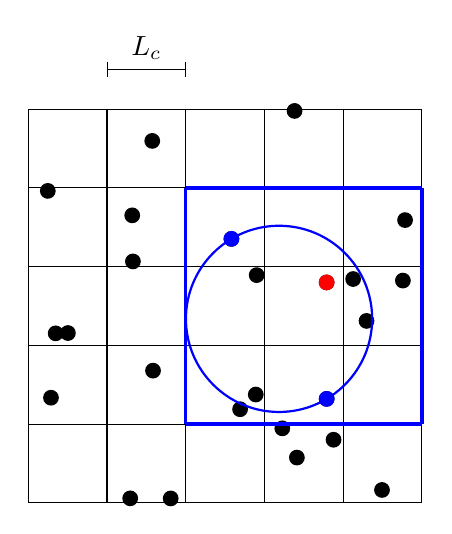
\begin{tikzpicture}
    \draw[|-|] (1,5.5) -- node[above] {$L_c$} (2,5.5);
    %~ \draw[|-|] (-0.5,3) -- node[left] {$L_c$} (-0.5,4);
    \foreach \x in {0,1,...,5}{
        \draw (0,\x) -- (5,\x);
        \draw (\x,0) -- (\x,5);
    }
    %random numbers generated by Python
    \foreach \x / \y in {0.28897762565/1.33479488842, 1.29507843519/0.0567389232558, 1.32094528703/3.65045643132, 2.90131976409/2.89143039453, 3.38227004393/4.97678250754, 4.78587153595/3.59043085053, 4.49289684902/0.16312339617, 2.88976245038/1.37508072608, 0.503908610931/2.15612491084, 4.29648323686/2.30979809325, 1.57506933975/4.5958939884, 3.41193951077/0.574638720997, 1.58494426782/1.67834825887, 3.87742721851/0.800878920581, 0.34861369265/2.15217676901, 3.78999774171/1.31996000053, 3.22671310651/0.945568165194, 2.58060642147/3.3521091272, 1.8091306587/0.055518765505, 4.12621981945/2.84187520295, 2.69064049175/1.18843544815, 0.248568008024/3.96126629448, 1.32959523341/3.0654517407, 4.7582022563/2.8223407318, 3.78979061396/2.79890572216}{
        \fill (\x, \y) circle(0.1);
    }
    %~ 2.58060642147/3.3521091272
    %~ 3.78999774171/1.31996000053
    \def\xa{2.58060642147}
    \def\ya{3.3521091272}
    \def\xb{3.78999774171}
    \def\yb{1.31996000053}
    \def\x{3.1853020815900002}
    \def\y{2.3360345638649997}
    \def\d{1.1823977163477497}
    \fill[blue] (\xa,\ya) circle(0.1);
    \fill[blue] (\xb,\yb) circle(0.1);
    \fill[red] (3.78979061396,2.79890572216) circle(0.1);
    \draw[blue,very thick] (2,1) -- (5,1);
    \draw[blue,very thick] (2,4) -- (5,4);
    \draw[blue,very thick] (2,1) -- (2,4);
    \draw[blue,very thick] (5,1) -- (5,4);
    \draw[blue,thick] (\x, \y) circle(\d);
\end{tikzpicture}

                                \end{figure}
                            }
                        }
                        \onslide<7>{
                                \begin{figure}[htbp]
                                    \centering
                                    \documentclass{standalone}
\usepackage{tikz}

\begin{document}
    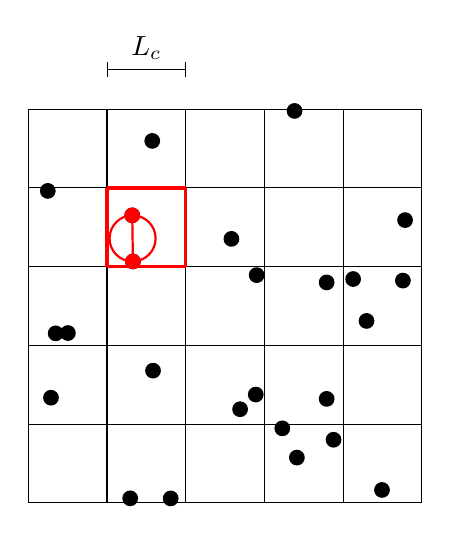
\begin{tikzpicture}
        \draw[|-|] (1,5.5) -- node[above] {$L_c$} (2,5.5);
        \foreach \x in {0,1,...,5}{
            \draw (0,\x) -- (5,\x);
            \draw (\x,0) -- (\x,5);
        }
        %random numbers generated by Python
        \foreach \x / \y in {0.28897762565/1.33479488842, 1.29507843519/0.0567389232558, 1.32094528703/3.65045643132, 2.90131976409/2.89143039453, 3.38227004393/4.97678250754, 4.78587153595/3.59043085053, 4.49289684902/0.16312339617, 2.88976245038/1.37508072608, 0.503908610931/2.15612491084, 4.29648323686/2.30979809325, 1.57506933975/4.5958939884, 3.41193951077/0.574638720997, 1.58494426782/1.67834825887, 3.87742721851/0.800878920581, 0.34861369265/2.15217676901, 3.78999774171/1.31996000053, 3.22671310651/0.945568165194, 2.58060642147/3.3521091272, 1.8091306587/0.055518765505, 4.12621981945/2.84187520295, 2.69064049175/1.18843544815, 0.248568008024/3.96126629448, 1.32959523341/3.0654517407, 4.7582022563/2.8223407318, 3.78979061396/2.79890572216}{
            \fill (\x, \y) circle(0.1);
        }
        %~ 1.32094528703/3.65045643132
        %~ 1.32959523341/3.0654517407
        \def\xa{1.32094528703}
        \def\ya{3.65045643132}
        \def\xb{1.32959523341}
        \def\yb{3.0654517407}
        \def\x{1.3252702602199999}
        \def\y{3.3579540860099999}
        \def\d{0.29253431833708793}
        \fill[red] (\xa,\ya) circle(0.1);
        \fill[red] (\xb,\yb) circle(0.1);
        \draw[red,very thick] (1,3) -- (2,3);
        \draw[red,very thick] (1,4) -- (2,4);
        \draw[red,very thick] (1,3) -- (1,4);
        \draw[red,very thick] (2,3) -- (2,4);
        \draw[red,thick] (\x, \y) circle(\d);
        \draw[red,thick] (\xa, \ya) -- (\xb, \yb) ;
    \end{tikzpicture}
\end{document}

                                \end{figure}
                        }
                    \end{overprint}
                \end{column}
            \end{columns}
        \end{frame}

\section{Methods}
    \subsection{Monte Carlo Simulations}
        \begin{frame}{Monte Carlo Simulations}
            \begin{itemize}[<+->]
                \item generate random states
                \item mesure observables of these states
                \item{ estimate observable \(O\) by
                    \begin{equation}
                        \avg{O} = \frac{1}{Z} \sum_i p_i O_i
                    \end{equation}
                }
            \end{itemize}
            \begin{itemize}[<+->]
                \item But there are states contributing more than others
                \item{ e.g.\ low \(H_{i}\) in canonical systems at low \(T\) with
                    \begin{equation}
                        p_{i} = e^{-\frac{H_{i}}{k_{B}T}}
                    \end{equation}
                }
            \end{itemize}
        \end{frame}

        \begin{frame}{Importance Sampling}
            \begin{itemize}[<+->]
                \item generate new states according to the known distribution \(p_{i}\)
                \item generate new states from former states
                \item{ Markov Chains
                    \begin{itemize}
                        \item Ergodicity\\
                                every state is reachable in finite time
                        \item Detailed Balance\\
                                in equilibrium the probability to reach a state is the same as the probability to leave the same state
                    \end{itemize}
                }
                \item note that the correlation of subsequent states has an effect on the errorbars\\
                    \(\to\) autocorrelation time \(\tau\)
            \end{itemize}
        \end{frame}

        \begin{frame}{Single Spin Flip Metropolis Update \cite{Metropolis1953}}
            \begin{equation}
                A(\mu \to \nu) =
                \begin{cases}
                    1                            & \Delta H \le 0 \\
                    \exp{\brac{-\beta \Delta H}} & \Delta H > 0
                \end{cases}.
            \end{equation}
        \end{frame}

        \begin{frame}{Wolff Cluster Update \cite{Wolff1989}}
            \begin{equation}
                P_{\mathrm{add}} = 1-\exp\brac{-2\beta J},
            \end{equation}
            \pause
            \begin{itemize}[<+->]
                \item very efficient at \(T_{c}\)
                \item but inferior to Metropolis at large and small \(T\)
            \end{itemize}
        \end{frame}

        \begin{frame}{Parallel Tempering \cite{ParallelTempering1986}}
            \begin{equation}
                P_{i,i+1}((E_i,T_i) \to (E_{i+1},T_{i+1})) = \min\brac{1,e^{\brac{\brac{E_{i+1}-E_i}\brac{\frac{1}{T_{i+1}}-\frac{1}{T_i}}}}}
            \end{equation}
            \begin{columns}[b]
                \begin{column}{5cm}
                    \begin{figure}[htbp]
                        \centering
                        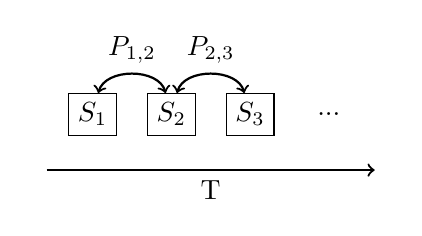
\begin{tikzpicture}
    \node[draw,rectangle] (a) {$S_1$};
    \node[draw,rectangle,right of=a] (b) {$S_2$};
    \node[draw,rectangle,right of=b] (c) {$S_3$};
    \node[rectangle,right of=c] (d) {...};

    \node[rectangle,below left of=a] (A) {};
    \node[rectangle,below right of=d] (D) {};
    \draw[thick,->] (A) edge node[below] {T} (D);

    \draw[thick,<->] (a) edge[out=75,in=105] node[above] {$P_{1,2}$} (b);
    \draw[thick,<->] (b) edge[out=75,in=105] node[above] {$P_{2,3}$} (c);
    %~ \draw[thick,<->] (c) edge[out=80,in=100] node[above] {$P_{..}$} (d);
\end{tikzpicture}

                        \caption
                        {
                            Swapping the spin configurations.
                        }
                    \end{figure}
                \end{column}
                \pause
                \begin{column}{6cm}
                    \begin{figure}[htbp]
                        \centering
                        \documentclass{standalone}
\usepackage{tikz}

\begin{document}
    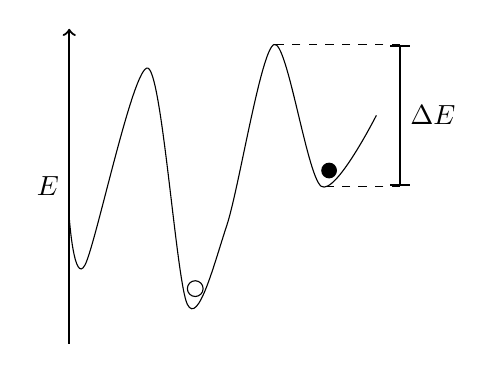
\begin{tikzpicture}
        %~ \draw[thick,->] (0,0) -- node[below] {$T$} (6,0);
        \draw[thick,->] (0,0) -- node[left] {$E$} (0,4);

        \draw plot [smooth] coordinates {(0,1.6) (0.2,1) (1,3.5) (1.5,0.5) (2,1.5) (2.6,3.8) (3.2,2) (3.9,2.9)};

        \fill (3.3,2.2) circle(0.1);
        \draw (1.6,0.7) circle(0.1);

        \draw[thick,|-|] (4.2,2) -- node[right] {$\Delta E$} (4.2,3.8);
        \draw[dashed] (4.2,2) -- (3.2,2);
        \draw[dashed] (4.2,3.8) -- (2.6,3.8);
    \end{tikzpicture}
\end{document}

                        \caption
                        {
                            Sketch of an energy landscape.
                        }
                    \end{figure}
                \end{column}
            \end{columns}
        \end{frame}

\section{Results}
    \begin{frame}{Details}
        \begin{itemize}[<+->]
            \item Aim: determining the dependence from \(T_{c}\) on \(\sigma\)
            \item \(10^{4} (L\in\{16,32\})\) or  \(5\cdot 10^{3} (L\in\{64,128\})\) uncorreltated measurements of \(O\) to get \(\avg{O}\)
            \item on each of 100 randomly generated proximity graphs to get \(\overline{\avg{O}}\){}
            \item \(m = \frac{1}{N} \sum_{i} s_{i}\)
            \item \(E = \frac{1}{N} H\)
        \end{itemize}
    \end{frame}

    \subsection{Finite Size Scaling}
        \begin{frame}{Finite Size Effects}
            \begin{columns}[t]
                \begin{column}{5cm}
                    \begin{itemize}[<+->]
                        \item \(T_{c}\) defined for \(L \to \infty\)
                        \item here: to ways to determine \(T_{c}\) are used
                        \item Finite Size Scaling to collapse the data
                        \begin{itemize}[<+->]
                            \item yields also critical exponents
                        \end{itemize}
                        \item Intersection of the Binder Cumulant
                        \begin{itemize}[<+->]
                            \item very simple and easy to automate
                        \end{itemize}
                    \end{itemize}
                \end{column}
                \begin{column}{6cm}
                    \begin{figure}[htbp]
                        \centering
                        \includegraphics[width=1\textwidth]{plots/meanM}
                        \caption
                        {
                            Finite Size Effects
                        }
                    \end{figure}
                \end{column}
            \end{columns}
        \end{frame}

    \subsection{Critical Exponents}

    \subsection{Critical Temperature}

\section{References}
    \begin{frame}[allowframebreaks]
        \bibliography{lit}
        \bibliographystyle{amsplain}
    \end{frame}

\end{document}
